\documentclass{../../ece-report}

\usepackage{subcaption}

\memostudent{Ty Davis}
\memotitle{Lab 3 - Diode Based Limiting and Clamping Circuits}
\memocourse{ECE 3110}
\memodate{\today}

\newcommand{\twosubfigures}[6]{
  \begin{subfigure}{0.45\textwidth}
    \includegraphics[width=\textwidth]{#1}
    \caption{#2}
    \label{#3}
  \end{subfigure}
  \begin{subfigure}{0.45\textwidth}
    \includegraphics[width=\textwidth]{#4}
    \caption{#5}
    \label{#6}
  \end{subfigure}
}

\begin{document}

\maketitle

\section{Introduction}

In this report we analyze the circuits shown in Fig.~\ref{fig:ciruits}
through computer simulation, then compare the results
with measurements we record in the lab with the oscilloscope.
All of these circuits are commonly used diode circuits
and will produce unique outputs.

\begin{figure}[h!]
  \centering
  \begin{subfigure}{.45\textwidth}
    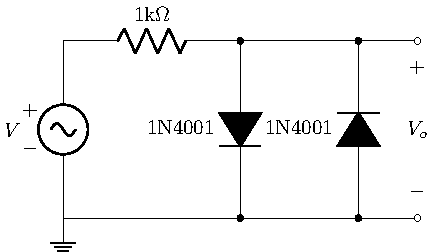
\includegraphics[width=\textwidth]{../circuits/circuit_a.pdf}
    \caption{Limiter Circuit}
    \label{fig:circuit_a}
  \end{subfigure}
  \begin{subfigure}{.45\textwidth}
    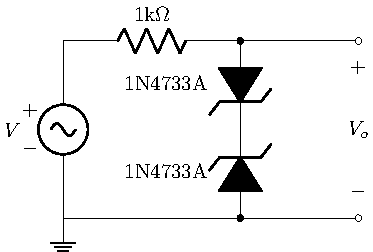
\includegraphics[width=\textwidth]{../circuits/circuit_b.pdf}
    \caption{Zener Diode Limiter Circuit}
    \label{fig:circuit_b}
  \end{subfigure}
  \begin{subfigure}{.45\textwidth}
    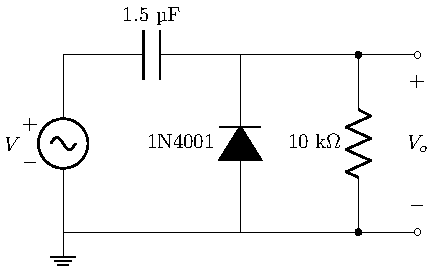
\includegraphics[width=\textwidth]{../circuits/circuit_c.pdf}
    \caption{Clamping Circuit}
    \label{fig:circuit_c}
  \end{subfigure}
  \begin{subfigure}{.45\textwidth}
    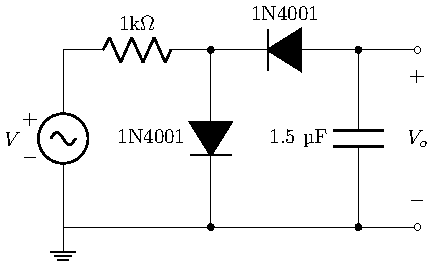
\includegraphics[width=\textwidth]{../circuits/circuit_d.pdf}
    \caption{Voltage Doubler Circuit}
    \label{fig:circuit_d}
  \end{subfigure}
  \caption{Circuits that are used in this lab.}
  \label{fig:ciruits}
\end{figure}

\section{Limiter Circuit}

\begin{figure}[h!]
  \centering
  \twosubfigures{../plots/circuit_a/pdf/a_sim_xy.pdf}{Simulated}{fig:simulated}
                {../plots/circuit_a/pdf/a_meas_xy.pdf}{Measured}{fig:measured}
  \caption{Limiter Circuit Simulation and Measurements}
  \label{fig:limiter_results}
\end{figure}

\section{Zener Diode Limiter Circuit}

\begin{figure}[h!]
  \centering
  \twosubfigures{../plots/circuit_b/pdf/b_sim_xy.pdf}{Simulated}{fig:simulated}
                {../plots/circuit_b/pdf/b_meas_xy.pdf}{Measured}{fig:measured}
  \caption{Limiter Circuit Simulation and Measurements}
  \label{fig:zener_limiter_results}
\end{figure}

\section{Clamping Circuit}

\begin{figure}[h!]
  \centering
  \twosubfigures{../plots/circuit_c/pdf/c_sim_trans.pdf}{Simulated}{fig:simulated}
                {../plots/circuit_c/pdf/c_meas_trans.pdf}{Measured}{fig:measured}
  \caption{Limiter Circuit Simulation and Measurements}
  \label{fig:clamped_results}
\end{figure}


\section{Voltage Doubler Circuit}

\begin{figure}[h!]
  \centering
  \twosubfigures{../plots/circuit_d/pdf/d_sim_trans.pdf }{Simulated}{fig:simulated}
                {../plots/circuit_d/pdf/d_meas_trans.pdf}{Measured}{fig:measured}
  \caption{Limiter Circuit Simulation and Measurements}
  \label{fig:doubler_results}
\end{figure}

\section{Conclusion}

\end{document}
